\documentclass{article}
\usepackage{graphicx}
\graphicspath{ {images/} }
\usepackage[letterpaper, portrait, lmargin=1in, rmargin=1in, tmargin=1in, bmargin=1in]{geometry}
\usepackage{color}
\usepackage{setspace}
\doublespacing

\title{External Validity of Experimental Social Preference Games}
\author{Sarah Xu}
\date{16 December 2017}

\begin{document}

\maketitle

\section{Introduction and Literature Review}

The standard economic model assumes actions are motivated purely by self-interest. However, it\rq s clear from simple observation that people actually care about the wellbeing of others: social programs exist, people volunteer, and people donate. If someone is not solely motivated by material self-interest but also cares about the material payoffs of others, we say that the person has social preferences. The last few decades have seen a strong increase of interest in social preferences, with numerous research studies providing evidence of social preferences. Papers have identified different aspects of social preferences such as altruism, social welfare, inequality aversion, and reciprocity (e.g., Charness and Rabin 2000; Fehr and Schmidt 1999; Andreoni and Miller 2002; Rabin 1993; Fisman, Jakiela, and Kariv 2014). 
 
When studying social preferences, the typical approach is to conduct experiments in a laboratory setting. Participants play experimental games, and receive monetary incentives that are aligned with the payoffs of the games. The experimental games allow researchers to target the different aspects of social behavior, and the laboratory setting strips the games from contextual features. Below are common games used to study social preferences: 

\begin{itemize}

\item{Dictator Game}: Two-player game where the first player (the dictator) receives an endowment, \textit{m}. The dictator chooses how to split the amount between themselves and the second player (the receiver) so that \(\pi_{s} + \pi_{o} = \textit{m}\), where \(\pi_{s}\) is how much is kept and \(\pi_{o}\) is how much is given.
\item{Ultimatum Game}: Two-player game where two players bargain over a fixed endowment, \textit{m}. The first mover divides the sum, so that \(\pi_{s} + \pi_{o} = m\). The second mover chooses to either accept or reject the offer. If accepted, the proposal is implemented. If rejected, neither player receives any money.
\item{Trust Game}: Two-player game where the first player receives an endowment, \textit{m}, and proposes how to divide the endowment between themselves and the second mover so that \(\pi_{s} + \pi_{o} = m\). The second player (the responder) receives \(k\pi_{o}\), where k $>$ 1, and decides how much of the endowment to return to the first mover. 
\item{Public Goods Game}: N-player game where each player receives the same sum of money, \textit{m}, and simultaneously decides how much to put into a public fund. The payoff function is given by \( P_{i} = m - g_{i} + \beta \sum_{n=1}^{N} g_{j} \) , where \(g_{i}\) is the amount that player \textit{i} donated to the fund, \(\beta\) is the marginal payoff of the public fund (0$<$\(\beta\)$<$N\(\beta\)), and \(\sum_{n=1}^{N}g_{j}\) is the sum of the individual donations to the public fund. 

\end{itemize}

There is an abundance of literature that study social preferences using experimental games. For example, Fehr and Schmidt (1999) used ultimatum and dictator games to identify whether people have inequality aversion, Berg et al (1995) employed trust games to provide evidence of reciprocity, and Hermann, Thoni, and Gachter (2008) used public goods game to provide evidence of punishment and reciprocity. This methodology has become one of the building blocks of experimental and behavioral economics. 
 
However, lab experiments also have its disadvantages. They are abstract and remote from realistic situations. Therefore, an important question is the extent to which the experimental games approach to social preferences can be generalized to real world situations. Human behavior may be influenced by a variety of factors that differ between practical and lab setting. One issue is that in a lab setting, the subject's actions are under the scrutiny of the researcher. Hoffman et al (1994) found that almost 50\% of their subjects donated at least \$3 (out of a \$10 pie) under a normal dictator game. However, the authors then implemented a ``double-blind'' treatment where both experimenter and other subjects couldn\rq t observe the dictator\rq s actions, and found that only 16\% of subjects gave at least \$3. There are other papers that also find that subjects are more prosocial in the lab than they are in the field (List, 2006; Gneezy et al., 2004). People are also influenced heavily on the context of the situation. Ross and Ward (1996) found that simply calling a prisoner's dilemma game a ``community'' or ``Wall Street'' game wildly varied each treatment group\rq s rates of defection. There are also other studies that find that slightly changing the narrative could result in significant changes in behavior (Burnham, McCabe, and Smith, 2000; and Gintis, 2001). Lastly, studies find evidence that varying the level of stakes may lead to significantly different behaviors. For example, Carpenter, Verhoogen, and Burks (2005) find that increasing the stakes from \$10 to \$100 decreased the median offer in the dictator game from 40\% to 20\%. Slonim and Roth (1998) and Parco, Rapoport, and Stein (2002) also find that higher stakes leads to significantly different results than with lower stakes. Interestingly, though, Cherry, Frykblom, and Shogren (2002) find no differences in offers when increasing the stakes from \$10 to \$40. Scrutiny, context, and stakes are only a few factors that can lead to deviations in behavior. Levitt and List (2007) discuss other factors that can lead to deviations in behavior between laboratory and field setting. 
 
The fact that varying factors such as scrutiny, context, and stakes can yield significant differences in behavior calls into question the external validity of using experimental games in a laboratory setting to study social preferences. There are a few studies that have examined how subjects\rq \ behavior in a lab setting is compared to the same subjects\rq  behavior in a real world situation. Baran et al (2010) compared MBA alumni donations to their university with their reciprocity behavior when playing a trust game in the lab. They find that that the in-lab behavior predicts university donations. Franzen and Pointner (2013) compare behaviors from university students participating in standard dictator games and their actions when receiving a misdirected letter containing money. The authors find that subjects who showed prosocial behavior in the lab returned the misdirected letters more often than subjects who were selfish in the lab. Englmaier and Gebhardt (2010) conducted field experiments with university students, comparing free riding behavior at the university library with free riding behavior when participating in a public goods experiment. The authors find statistically significant correlation between field and lab measures. There are also studies using non-student subjects. Fehr and Leibbrandt (2011) conducted public goods games with Brazilian fishermen, and find that fishermen who are more cooperative in the games were also less likely to exploit the communal fishing grounds. Karlan (2005) compared Peru inhabitants\rq  \ trust game behaviors to their repayment behavior of micro loans, and finds correlation between game results and repayment behavior. 

On the other hand, there are a number of papers that find lab behavior has no predictive power for field behavior. Goeschl et al (2015) examined university students\rq \ behavior in two different tasks: a public goods game and their contributions to a task about reducing CO2 emissions. The authors find that behavior in both tasks is uncorrelated. Hill and Gurven (2004) carried out ultimatum and public goods games on Paraguay Ache Indians. They compared the behaviors to observed food production and sharing patterns to individuals outside the nuclear family and found no significant relationships to lab behavior. Gurven and Winking (2008) used Tsimane forager-horticulturalists in Bolivia as their subjects, and compared behavior when playing dictator and ultimatum games to their food-sharing behavior. The authors find no relation between the two measures. Voors et al (2012) studied farmers in Sierra Leone, and compared their behavior in a public goods game to their behavior when asked to contribute to a real community public good. They find no meaningful correlation in behavior between the lab and field measures. With other studies finding statistically significant, not statistically significant, and mixed results, the currently accumulated evidence is ambiguous. This is clear evidence that justifies further research is needed. 

 
While the literature on comparing the behavior of a single individual in both the lab and field, Galizzi and Navarro-Martinez (2017) argue that the studies compareonly one social preference game to one specific field measure. The abstract and context-free nature of the games makes it difficult to theoretically map the games to the field measure, and so it is crucial to have a more systematic approach. The authors proceed to carry out their own study, comparing behavior in various games with behaviors elicited in various field situations. Participants answered a questions about social behaviors exhibited in the past, played various f social preference games, and encountered naturalistic field situations related to social preferences. Examples of the field situations included a research assistant asking for help carrying boxes down the stairs, asking to use the participant\rq s phone to make a brief phone call, asking for donations to a children\rq s charity, asking for donations to an environmental charity, or asking for donations to the lab\rq s research fund. The authors\rq  overarching conclusion is that behavior when playing the experimental games does a poor job predicting both the survey questions and the field behaviors. They do note, however, that more systematic studies are needed to draw a definite conclusion. For example, future studies could look at other field situations or other game structures. 

It is critical to think about why some experiments found correlations and some did not, in order to inform the design of our current experiment. An underlying theme for those experiments that found no correlations is higher stakes. Voors et al (2012) note that an important difference between the lab and field experiment are that the stakes are much higher in the field experiment: a month\rq s wage versus a day\rq s wage, and the public good affected the entire village rather than two other players. In Gurven and Winking (2008)\rq s study, there are different stakes between the experimental and field measures. The authors note that ``money is fungible and easier to hide than agricultural produce or meat and is shared differently than other resources''. In addition, stakes are especially higher for food-sharing behavior since food-sharing is heavily ingrained in the culture. Lastly, while playing the experimental games for Hill and Gurven (2004)\rq s study, participants expressed worry that their choices would make the receiver upset. In particular, the tribal group\rq s culture was heavily focused on community, and was well known for extensive food sharing (which was the field measure the authors used). Perhaps the participants didn\rq t want to risk their choices creating any tension in their community, and getting punished with less food sharing and cooperation. For the last two papers, the stakes were a result of high scrutiny and low anonymity since it was easy for community members to find out the choices each subject made. For our design, an important aspect is that participants will play the games in their own time and location to ensure no scrutiny and high anonymity. 

Similar to Galizzi and Navarro-Martinez (2017), I will recruit Wesleyan University students to play various experimental games and non-incentivized social preference questions.  A major criticism of the design is how the authors executed their field measures. Since the setup occurs as the participants are exiting their lab session, it\rq s hard to believe that the participants did not connect the encounters to the research lab, especially since they previously answered questions similar to the current event. Therefore it is better to use a natural, far-removed situation. For my paper, I will be using donations of seniors and recent alumni to Wesleyan University. Donors can choose what area their donations will go towards (for example financial aid, academic programming and faculty support, and or student activities). These different donation options can be related to some behavioral constructs. For example, donating may represent altruism and reciprocity, and donating to financial aid may represent inequality aversion. 
 
Ultimately, my paper will add to the growing literature on the external validity of experimental social preference games. By comparing my results with those of past studies, I can contribute to the discussion on whether experimental games are a useful tool to examine social preferences. In addition, my paper can perhaps trigger interest into future studies on the external validity of using lab experiments for other behavioral economics topics. 


\section{Methods}

The goal of this study is to evaluate the external validity of experimental social preference games to behaviors in the field, and if perhaps another tool (in this case, survey questions) can better predict social preferences exhibited in the field. The participants will be presented with two sets of tasks: (1) survey questions regarding past social behavior, and (2) incentivized social preference games. The field measure that will be compared to participants\rq lab results will be their Wesleyan donations. 
 
Both instruments will be sent via a single link in an email, and participants will be able to play the experimental games and answer the survey and non-incentivized questions online remotely (images of the computerized games and questions are in Figure 1). All the games are computerized, and they were programmed and implemented using Qualtrics. 
 
The participants will receive a unique identifier, as well as detailed instructions about the tasks they will complete in the session. They will also be informed that, with their permission, their major, class year, and Wesleyan donations information will be released to me. 


\subsection{Self-reported measures of past social behaviors}

Participants report on social behaviors exhibited in the past. The questions are loosely based off of the Self-Report Altruism (SRA) scale introduced by Rushton, Chrisjohn, and Fekken (1981). 

The survey is comprised of 15 items, and participants report how frequently they have one each item in the past. Participants rate each statement on a scale from 1 (``never'') to 5 (``very often''). Examples include: ``I have donated money at the cash register when buying groceries'', ``I have pointed out a clerk\rq s error (at the supermarket, at a restaurant) in undercharging me'', and ``I have donated instead of sold my clothes/used items''. A full list of the 15 items is displayed in Table 1. 

\subsection{Incentivized social preference games}

Participants also play various social preference games. I will use four games that are widely used in behavioral economics to study social preferences: generalized dictator game, ultimatum game, trust game, and public goods game. For the ultimatum and trust games, each participant will have the opportunity to play the role of the both first mover and second mover.

Since they are completing the games at their own availability, they will not be randomly matched with other participants. Instead, if the game requires two players, the second player will see a list of all possible options, and are prompted for their choice for each option listed (further discussion about the strategy method is in Section 2.2.1). 

Participants will receive instructions for the various games they will be playing. In order to incentivize completion of both the games and survey questions, as well as elicit honest decisions, participants will be eligible for a prize upon completion of the study. All games use "tickets" as the experimental currency unit, and participants' chances of winning a prize will be dependent on their total tickets earned in the experimental games. I will explain the payment process in further detail in Section 2.4.1. 

Below are the different games each participant will play: 

\begin{itemize}

\item{Generalized Dictator Game}:  Each participant (playing as Player 1) is asked to make a series of choices about how to divide tickets between themselves and an anonymous, random Player 2. Every ticket that Player 1 earns will be worth 1, 2, 3 or 4 tickets, depending on the choice. Similarly for the earnings of Player 2. The design is based off of Andreoni and Miller (2002).
\item{Ultimatum Game}: 
	\begin{itemize}
		\item{Player 1}: Each participant plays as the proposer, and is endowed with 10 tickets. They decide how much of their endowment to send to an anonymous, random Player 2. They are told that Player 2 may or may not reject the allocation. If the allocation is rejected, neither player receives any tickets.
		\item{Player 2}: Each participant is now the responder. They are given a list from 0 tickets to 10 tickets (in 1-ticketincrements), and are asked whether they accept or reject each listed amount.
	\end{itemize}
\item{Trust Game}:
	\begin{itemize}
		\item{Player 1}: Each participant plays as the proposer, and is endowed with 10 tickets. They decide how much of their endowment to send to an anonymous, random Player 2. The amount sent over is multiplied by three. Player 2 then decides how many tickets to return. 
		\item{Player 2}: Now each participant is the responder. They receive a list of all ten possible multiplied amounts that Player 1 could have chosen to send. For each amount, they are prompted to enter the number of tickets they would like to return.
	\end{itemize}
\item{Public Goods Game}: Each participant is endowed with 10 tickets and have to decide how much of their endowment to contribute to a group fund with one other anonymous, random participant. The total tickets in the group fund is multiplied by 2 and divided evenly between the two players.

\end{itemize}

These experimental games address many of the main behavioral constructs that explain social preferences. Some constructs include: altruism (dictator game, public goods game); positive reciprocity (trust game responder); negative reciprocity (ultimatum game responder); trust (trust game proposer); cooperation (public goods game); and inequality aversion (all games). 

\subsubsection{Strategy Method}

Each participant has the opportunity to be both proposer (Player 1) and responder (Player 2) in each game. When the participant is the responder, the strategy method is used: the participant has to make decisions for all possible situations. For example, as the responder in the trust game, the participant has to decide how much money they will send back for all possible amounts that were given to them by the proposer. 

There are several reasons why the strategy method is employed. First, as mentioned previously, participants complete the experimental games in their own time, so participants will not be paired up while they are playing. Instead, they will be randomly paired at a later period. Therefore it is useful to have all of Player 2\rq s potential choices so that payoffs can be determined. Most importantly, the strategy method gives more information. Using the strategy method will provide all returned amounts for all possible donated amounts in the ultimatum game. In the trust game, the minimum donated amount that the responder will accept would be provided. 

\subsection{Field Measure}

Each participant\rq s Wesleyan donations information will be accessed upon their informed consent and completion of the survey and games. 

Wesleyan donations can represent different aspects of social preferences. Whether a participant donates or not can represent altruism. Donating can also represent reciprocity, since seniors/recent alumni are giving back to the university that provided them four years of education and opportunities, as well as represent cooperation and trust. In addition, donors are able to target what area their donations can go towards. For example, donating towards Financial Aid can represent inequality aversion, since Financial Aid makes the Wesleyan experience possible for talented, low-income students who might not otherwise be able to attend.  

A main feature of my design is that the donations information is a naturalistic environment that is far-removed from the experiment, which provides a more accurate field measure. I previously mentioned that Galizzi and Navarro-Martinez (2017)\rq s design is unsatisfactory since their subjects encountered the field experiment shortly after completing the lab experiments. I believe that it is not too difficult to link the two situations together. In my design, participants\rq \ donations behavior is not affected by their participation in the lab at the time. 

I chose to use the generalized dictator game, ultimatum game, trust game, and public goods game because each game can be mapped to donations behavior. First, the very nature of donating represents altruism - therefore, the generalized dictator game and proposers for the ultimatum and trust games are expected to be correlated with donating. In addition, inequality aversion can also explain why seniors and alumni donate: they want future students, perhaps especially those on financial aid, to be provided with the best opportunities. Dictators in the generalized dictator game, proposers in the ultimatum and trust games, and players in the public goods game can also represent inequality aversion.  Donating to one's university may also represent reciprocity, which is represented by the responders in the ultimatum and trust games. Lastly, the public goods game can also be mapped to donating because it represents cooperation: seniors and alumni will give if they believe that others are donating as well. 
	
\subsection{Participants and Sessions}
Emails containing the link to access the online experimental games and survey questions will be sent to all current Wesleyan University seniors and recent alumni (those who graduated within 5 years) in early January. They will have until mid-February to participate. The participants are those who volunteer to open the email link, provide consent for us to receive their major, class year, and Wesleyan donations data, and complete both the survey questions and social preference games. Besides soliciting seniors and recent alumni to participate, I use no other eligibility or exclusion criteria to select participants.

\subsubsection{Payment}
For each game, participants will be randomly paired, and payoffs will be determined. For each pair in the ultimatum game and trust game, one participant will be randomly assigned to their Player 1 choices, and the other participant will be assigned to their Player 2 choices. If the generalized dictator game is chosen, one player will be randomly assigned as the dictator, and the other player will be the receiver. However many tickets each participant earns in the end will correspond with the number of tickets they will have in the lottery. There will be ten lottery winners, and each winner will receive \$100. Winners will be contacted through email. 

Below are descriptions on how payoffs will be determined for each game: 

\begin{itemize}

\item Generalized dictator game: Participants will be paired up randomly. In each pair, one player will be randomly selected as the dictator, and the other will be the receiver.  Since the generalized dictator game consists 11 different sets of endowment and prices of giving, one set will be randomly picked for payoffs.

\item Ultimatum game: Participants will be randomly matched. For each pair, one participant will be randomly assigned to their choice when playing Player 1, and the other participant will be assigned to their choices when playing as Player 2. For example, if Player 1 chooses to give 4 tickets but Player 2 chooses not to accept that amount, then both players will receive nothing. But if Player 1 does accept that amount, then Player 1 will receive 6 tickets and Player 2 will receive 4 tickets.

\item Trust game: Participants will be randomly matched. For each pair, one participant will be randomly assigned to their choice when playing Player 1, and the other participant will be assigned to their choices when playing as Player 2, and payoffs will be determined. For example, if Player 1 chose to give 2 tickets to Player 2, then the multiplied amount is 6 tickets. Given being offered 6 tickets, if Player 2 chose to give back 1 ticket, then ultimately Player 1 will earn 9 tickets and Player 2 will earn 5 tickets.

\item Public goods game: Participants will be randomly paired up. The overall tickets in the public fund will be multiplied by 2 and divided evenly. Thus each participant will receive their remaining tickets plus the divided amount from the public fund.

\end{itemize}

\section{Analysis}

After gathering all experimental, survey, and donations data, I will be running two regression models:
\begin{equation}
donations= \beta_{0} + \beta_{1} GDG_{equity}+ \beta_{2} GDG_{efficiency} + \beta_{3} UG1 + \beta_{4} UG2 + \beta_{5} TG1 + \beta_{6} TG2 + \beta_{7} PGG
\end{equation}
\begin{equation}
donations = \beta_{0} + \beta_{1} SRA
\end{equation}
Since the generalized dictator game consists of 11 different sets of endowments and prices of giving, each participant's giving preferences will be represented using the constant elasticity of substitution (CES) utility function, written as: \\

\(u(\pi_{s}, \pi{o}) = [\alpha\pi_{s}^{\rho} + (1-\alpha)\pi_{o}^{\rho}]^{1/ \rho }\) \\

\noindent
where \(\alpha\) measures the weight on the payoff to self (i.e. propensity to share, or equity-minded) , and \(\rho\) indicates the willingness to trade off payoffs to self and other in response to price changes (i.e. utilitarian preferences, or efficiency-minded). Using the Lagrange function maximize utility subject to a budget constraint: \\

max \(u(\pi_{s}, \pi{o}) = [\alpha\pi_{s}^{\rho} + (1-\alpha)\pi_{o}^{\rho}]^{1/ \rho }\) such that \(\pi_{s} + p\pi_{o} = m\) \\

\(\mathcal{L} = u(\pi_{s}, \pi{o}) = [\alpha\pi_{s}^{\rho} + (1-\alpha)\pi_{o}^{\rho}]^{1/ \rho } + \lambda (m-\pi_{s}-p\pi_{o})\) \\

\(\frac{\frac{\partial \mathcal{L}}{\partial \pi_{s}}}{\frac{\partial \mathcal{L}}{\partial \pi_{o}}} = \frac{\frac{1}{\rho}[\alpha\pi_{s}^{\rho} + (1-\alpha)\pi_{o}^{\rho}]^{\frac{1}{\rho} -1}[\alpha\rho\pi_{s}^{\rho-1}]-\lambda}{\frac{1}{\rho}[\alpha\pi_{s}^{\rho} + (1-\alpha)\pi_{o}^{\rho}]^{\frac{1}{\rho} -1}[(1-\alpha)\rho\pi_{o}^{\rho-1}] - p\lambda} = 0 \ \ \longrightarrow \ \ \frac{\alpha\pi_{s}^{\rho-1}}{(1-\alpha)\pi_{o}^{\rho-1}} = \frac{1}{p} \ \ \longrightarrow \ \ \frac{\alpha}{1-\alpha}(\frac{\pi_{s}}{\pi_{o}})^{\rho-1} = \frac{1}{p}\) 
 \\
 
\noindent
Taking the natural logarithm on each side of the equation will result in the following regression:  \\

\indent
\( \ln(\frac{1}{p}) = \ln(\frac{\alpha}{1-\alpha})+(\rho-1)\ln(\frac{\pi_{s}}{\pi_{o}}) \)

\noindent
\\
For each participant, I will input their 11 \(\pi_{s}\), \(\pi_{o}\), and \textit{p} combinations into the equation. Running the equation will provide estimates for \(\beta_{0}\) and \(\beta_{1}\), which will correspond to estimates for \(\alpha\) and \(\rho\), respectively: \\

\(\hat{\beta_{0}} \rightarrow \hat{\alpha}, \ \  \hat{\beta_{1}} \rightarrow \hat{\rho} \) \\

Therefore in Model (1), \(GDG_{equity}\) is equal to \(\alpha\), the participant's sharing propensity, and \(GDG_{efficiency}\) is equal to \(\rho\), the participant's level of efficiency. 

UG1 represents the proposer\rq s pass rate (percentage of the initial endowment passed to the other player) in the ultimatum game, UG2 represents the minimum pass rate that the responder chooses to accept in the ultimatum game, TG1 represents the proposer\rq s pass rate in the trust game, TG2 measures the responder\rq s reciprocity: I will regress each participant's amount they pass back on the amount that was offered to them, and use the slope as a measure of reciprocity. PGG represents each player\rq s pass rate into the public fund. Lastly, SRA measures each participant\rq s self-report altruism score, which is calculated by summing across the 15 items (where ``Never''=0, ``Once''=1, ``More than once''=2, ``Often''=3, and ``Very often''=4).  

It makes sense that all \(\beta\)s, except for the \(\beta\) for UG2, will be positive. If the participant has a high sharing propensity, i.e. they place a high weight on giving, and a high efficiency level, i.e. they care a lot about total social welfare, then donations should be larger. As the participant\rq s pass rate for the ultimatum and trust game (coefficients for UG1 and TG1) increases, it indicates they have higher levels altruism, inequality aversion, or both, so donations should also increase. If the participant has higher levels of reciprocity, indicated by the coefficient on TG2, then donations should increase - the very nature of giving back to one's university is represented by reciprocity, so there should be a high, positive correlation between TG2 and measured donations. A higher pass rate into the public goods fund indicates higher levels of cooperation and altruism, so the coefficient on PGG should also be positive. Lastly, if the minimum pass rate accepted by the responder in the ultimatum game is high, this indicates that the responder is selfish - they will punish the proposer if the offer is not to their liking. Therefore it makes sense that the coefficient on UG2 is negative. 

First, I will run each model and examine how well each instrument predicts donations. With Model (1), I want to see which game best predicts donations behavior. For example, if I see that the dictator game and responder ultimatum game is statistically significant but all other games are not statistically significant, then perhaps further research could exclude using the other games when predicting charitable giving. This would certainly save researchers the time cost in programming the games, as well as make the experiment shorter (and therefore more attractive to participants). 

However, the overall goal is to determine which instrument is better at predicting the field measure. Along with Model (1) and Model (2), I will also be running:
\begin{equation}
donations=\beta_{0} + \beta_{1} GDG_{equity} + \beta_{2} GDG_{efficiency} + \beta_{3} UG1 + \beta_{4} UG2 + \beta_{5} TG1 + \beta_{6} TG2 + \beta_{7} PGG + \beta_{8}SRA
\end{equation}
I will examine each model's prediction errors, using mean squared errors (MSE). The MSE measures the average of the squares of the errors - that is, the difference between the estimator and what is estimated. MSE for Models (1), (2), and (3) is computed as: \\

\( MSE = \frac{1}{n}\sum_{i=1}^{n}(donations_{i}-\hat{donations}_{i})^{2} \) \\


Comparing Model (1) and Model (2)\rq s MSE will reveal whether incentivized experimental games or non-incentivized self-reported measures can better predict field measures on social preferences. Including Model (3) will tell us if, perhaps, having both instruments is better than only including one instrument.


\section{Importance and Benefits}

First, the findings in this experiment will add to growing literature and debate on whether experimental games are a useful tool to examine social preferences. The current accumulated evidence is mixed - some studies find that in-lab behavior is correlated to field behavior, while others do not find a significant relationship. However, the studies map only one experimental game to one field measure. My experience, which uses a variety of experimental games along with self-reported social behavior questions, therefore provides a systematic approach to uncovering the external validity of experimental social preference games. 

Along with adding to the literature on external validity of experimental social preference games, there is a potential policy implication with our findings from a research perspective. Experimental games are costly - not only is it expensive paying participants for attending the lab session and providing money aligned with the payoffs of the games (especially if more show up than expected), but it also takes a lot of time to program the experimental games. If experimental games do not better predict field measures, then perhaps eliminating experimental games and instead using non-incentivized survey questions is better for funding and logistical purposes. 

Finally, on a larger scale, this study can potentially spark interest into future studies into the external validity of other behavioral economics topics where lab experiments are also commonly used. For example, using experiments to study risk preferences and time preferences is common, so it will be interesting to see whether in-lab behavior is correlated to field measures, and perhaps adopting a systematic approach (comparing a variety of lab experiments to various field measures) can prove to be beneficial.
 \newpage
\begin{thebibliography}{9}

\bibitem{AndreoniMiller}
Andreoni, J., and Miller, J.H. (2002).
\textit{Giving according to GARP: An experimental test of the consistency of preferences for altruism}.
Econometrica, 70, 737-53.

\bibitem{Baran}
Baran, N.M., Sapienza, P., and Zingales, L. (2010).
\textit{Can we infer social preferences from the lab? Evidence from the trust game}.
NBER Working Paper 15654.

\bibitem{Benz}
Benz, M., and Meier, S. (2006).
\textit{Do people behave in experiments as in the field? Evidence from donations}.
Experimental Economics, 11, 268-81.

\bibitem{Berg}
Berg, J., Dickhaut, J.W., and McCabe, K.A. (1995).
\textit{Trust, reciprocity, and social history}.
Games and Economic Behavior, 90, 166-93.

\bibitem{Burnham}
Burnham, T., McCabe, K., Smith, V. (2000).
\textit{Friend-or-foe intentionality priming in an extensive form trust game}.
Journal of Economic Behavior \& Organization, 43, 57-73.

\bibitem{Carpenter}
Carpenter, J.P., Verhoogen, E., and Burks, S. (2005).
\textit{The effect of stakes in distribution experiments}.
Economics Letters, 86, 393-98.

\bibitem{CharnessRabin}
Charness, G., and Rabin, M. (2002).
\textit{Understanding social preferences with simple tests}.
Quarterly Journal of Economics, 117, 817-69.

\bibitem{Cherry}
Cherry, T., Fykblom, P., and Shogren, J. (2002).
\textit{Hardnose the Dictator}.
American Economic Review, 92(4): 1218-21.

\bibitem{Englmaier}
Englmaier, F., and Gebhardt, G. (2010)
\textit{The external validity of giving in the dictator gam: A field experiment using the misdirected letter technique}.
Governance and the efficiency of social systems (GESY), CESifo Working Paper No. 344.

\bibitem{FehrLeibbrandt}
Fehr, E., and Leibbrandt, A. (2011)
\textit{A field study on cooperativeness and impatience in the Tragedy of the Commons}.
Journal of Publicc Economics, 95, 1144-55.

\bibitem{FehrSchmidt}
Fehr, E., and Schmidt, K. (1999).
\textit{A theory of fairness, competition, and cooperation}.
Quarterly Journal of Economics, 114, 173-68.

\bibitem{Fisman}
Fisman, R., Jakiela, P., and Kariv, S. (2014).
\textit{The distributional preferences of Americans}.
NBER Working Paper.

\bibitem{Franzen}
Franzen, A., and Pointner, S. (2013)
\textit{The external validity of giving in the dictator gam: A field experiment using the misdirected letter technique}.
Experimental Economics, 16, 155-69.

\bibitem{Galizzi}
Galizzi, M., and Navarro-Martinez, D. (2017).
\textit{On the external validity of social preference games: a systematic lab-field study}.
Management Science.

\bibitem{Gintis}
Gintis, H. (2000).
\textit{Strong reciprocity and human sociality}.
Journal of Theoretical Biology, 206, 169-79.

\bibitem{Gneezy}
Gneezy, U., Haruvy, E., and Yafe, H. (2004).
\textit{The inefficiency of splitting the bill: A lesson in institutional design}.
The Economic Journal, 114(495), 265-80.

\bibitem{Goeschl}
Goeschl, T., Kettner, S.E., Lohse, J., and Schwieren, C. (2015)
\textit{What do we learn from public good games about voluntary climate action? Evidence from an artefactual field experiment}.
University of Heidelberg, Department of Economics Discussion Paper 595.

\bibitem{GurvenWinking}
Gurven, M., Winking, J. (2008).
\textit{Collective action in action: prosocial behavior in and out of the laboratory}.
American Anthropologist, 110(2), 179-190. 

\bibitem{Hermann}
Hermann, B., Thoni, C., and Gachter, S. (2008).
\textit{Anti-social punishment across societies}.
Science, 319, 1362-67.

\bibitem{HillGurven}
Hill, K., and Gurven, M. (2004)
\textit{Economic experiments to examine fairness and cooperation among the Ache Indians of Paraguay}.
In J. Henrich, R. Boyd, S. Bowles, C. Camerer, E. Fehr, and H. Gintis (Eds.),
Foundations of Human Sociality: Economic Experiments and Ethnographic Evidence from Fifteen Small-Scale Societies. Oxford University Press.

\bibitem{Hoffman}
Hoffman, E., McCabe, K., Shachat, K., and Smith, V. (1994).
\textit{Preferences, property rights, and anonymity in bargaining games}.
Games and Economic Behavior, 7(3): 346-80.

\bibitem{Karlan}
Karlan, D.S. (2005).
\textit{Using experimental economics to measure social capital and predict financial decisions}.
American Economic Review, 95, 1688-99.

\bibitem{Levitt}
Levitt, S., and List, J. (2007)
\textit{What do laboratory experiments measuring social preferences reveal about the real world?}.
Journal of Economic Perspectives, 21(2), 153-74.


\bibitem{List}
List, John. 2006.
\textit{The behavioralist meets the market: measuring social preferences and reputation effects in actual transactions}.
Journal of Political Economy, 114(51), 1-37.


\bibitem{Parco}
Parco, J., Rapoport, A., and Stein, W. (2002).
\textit{Effects of financial incentives on the breakdown of mutual trust}.
Psychological Science.

\bibitem{Rabin}
Rabin, M. (1993).
\textit{Incorporating fairness into game theory and economics}.
The American Economic Review, 83, 1281-1302.

\bibitem{Ross}
Ross, L., and Ward, A. (1996).
\textit{Naive realism in everyday life: Implications for social conflict and misunderstanding}.
Values and Knowledge, 103-35.

\bibitem{Rushton}
Rushton, J.P., Chrisjohn, R.D., and Fekken, G.C. (1981).
\textit{The altruistic personality and the self-report altruism scale}.
Personality and Individual Differences, 2, 293-302.

\bibitem{Slonim}
Slonim, R., and Roth, A. (1998).
\textit{Learning in high stakes ultimatum games: An experiment in the Slovak Republic}.
Econometrica, 66, 569-96.


\bibitem{Voors}
Voors, M., Turley, T., Kontoleon, A., Bulte, E., and List, J.A. (2012).
\textit{Exploring whether behavior in context-free experiments is predictive of behavior in the field: Evidence from lab and field experiments in rural Sierra Leone}.
Economic Letters, 114, 308-311.


\end{thebibliography}


\appendix
\section{Tables}

\begin{tabular}{ | p{12cm} | }
\hline
\multicolumn{1}{|c|}{SRA Questions List} \\
\hline
1. I have allowed someone to go ahead of me in line.\\
\hline
2. I have donated money at the cash register when buying groceries.\\
\hline
3. I have given money to a stranger (or an acquaintance I don\rq t know too well) in need.\\ 
\hline
4. I have donated instead of sold my clothes/used items.\\
\hline
5. I have donated to a charity.\\
\hline
6. I have donated blood.\\
\hline
7. I have done volunteer work for a charity/organization.\\
\hline
8. I have delayed an elevator/held door open for stranger(s).\\
\hline
9. I have lent an acquaintance that I don\rq t know too well with something of value to me (clothes, tools, etc).\\
\hline
10.  I have pointed out a clerk\rq s error (at a supermarket, restaurant) in undercharging me.\\
\hline
11. I have gone out of my way to meet with someone to help them with a task (e.g. help proofread their paper, listen to their presentation, etc). \\
\hline
12. I have helped carry a stranger\rq s belongings (e.g. groceries).\\
\hline
13. I have offered my seat on a bus/train to a stranger who was standing.\\
\hline
14. I have helped an acquaintance with moving in/ moving out of their dorm/apartment/house.\\
\hline
15. I have donated money/coins to the Salvation army bell-ringers.\\
\hline
\end{tabular}

\newpage


\section{Figures}
Figure 1: Online games and survey questions \\ \\
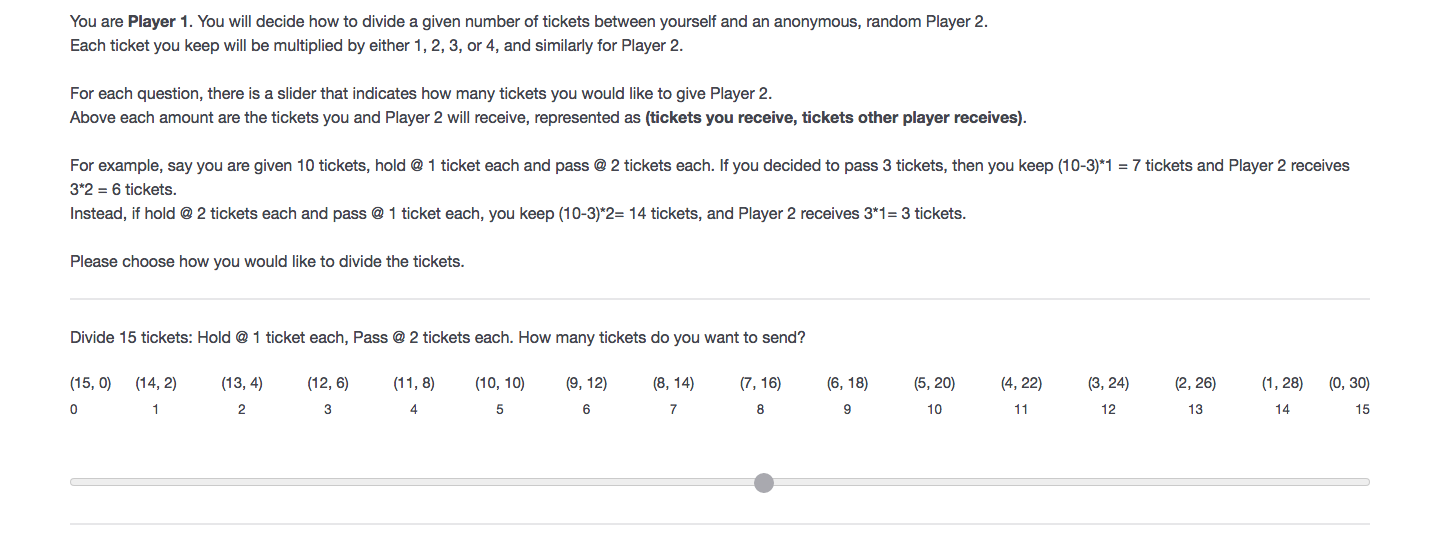
\includegraphics[scale=0.35]{gendict1}\\
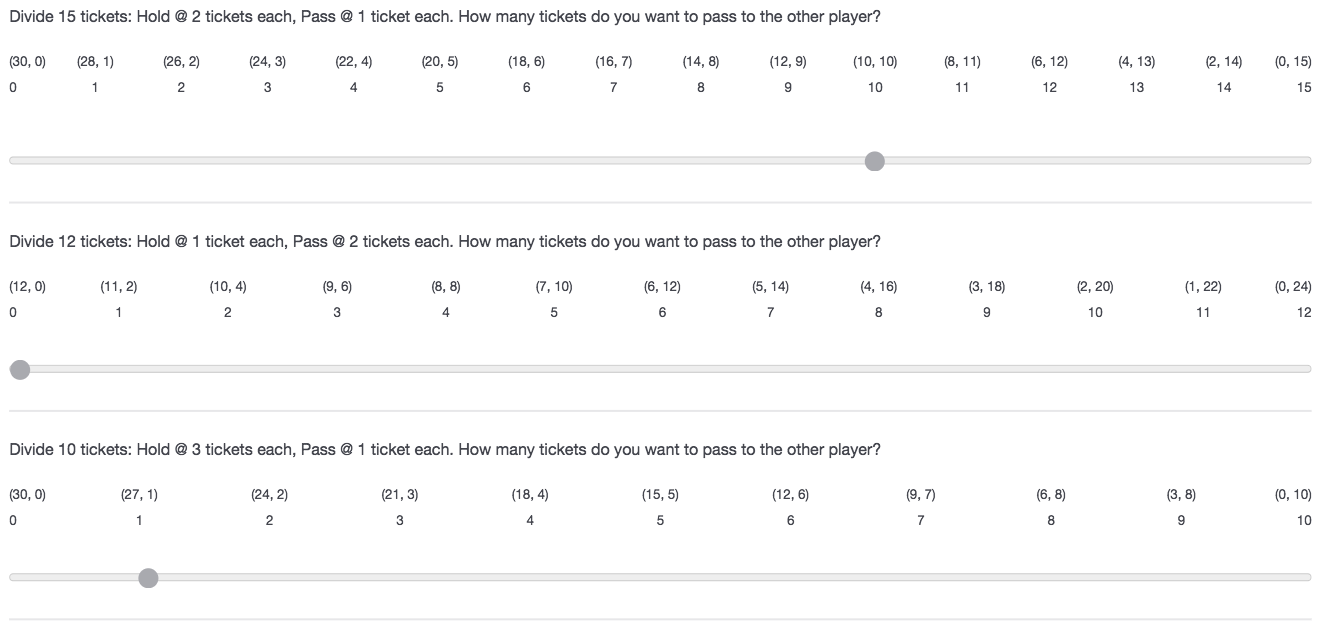
\includegraphics[scale=0.35]{gendict2}\\
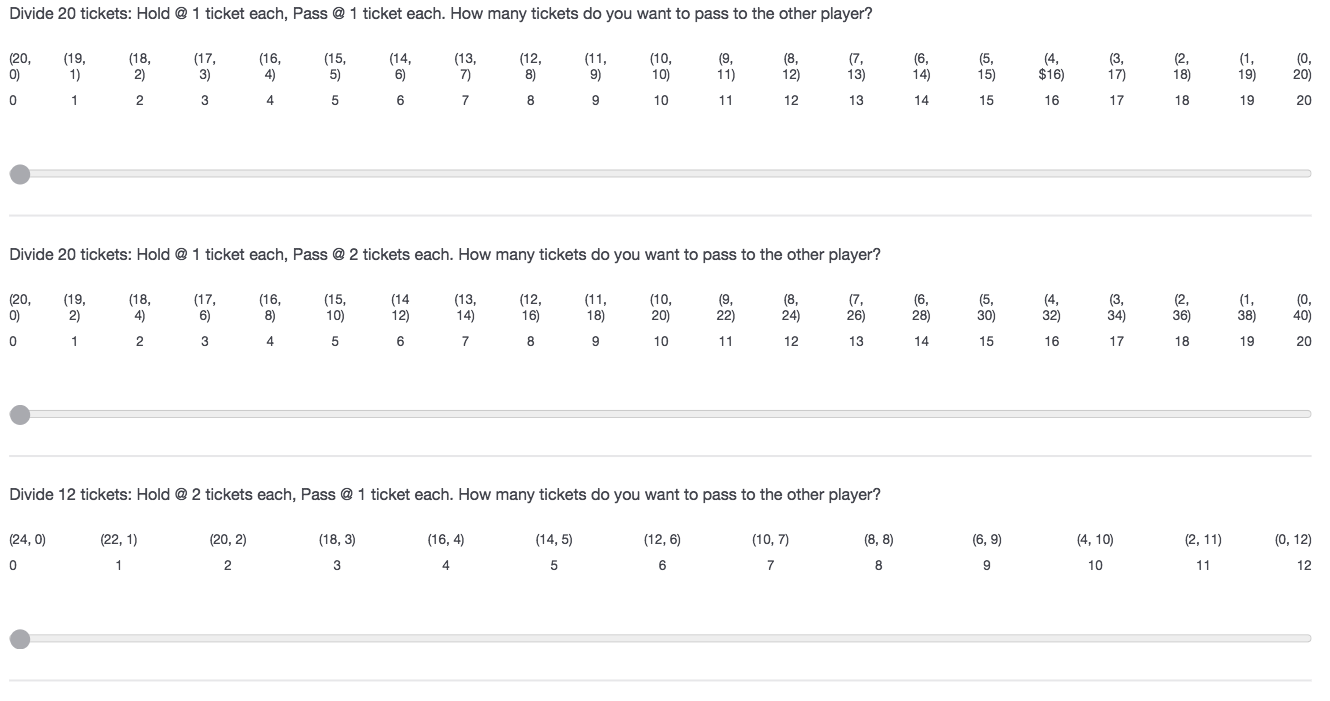
\includegraphics[scale=0.35]{gendict3}\\
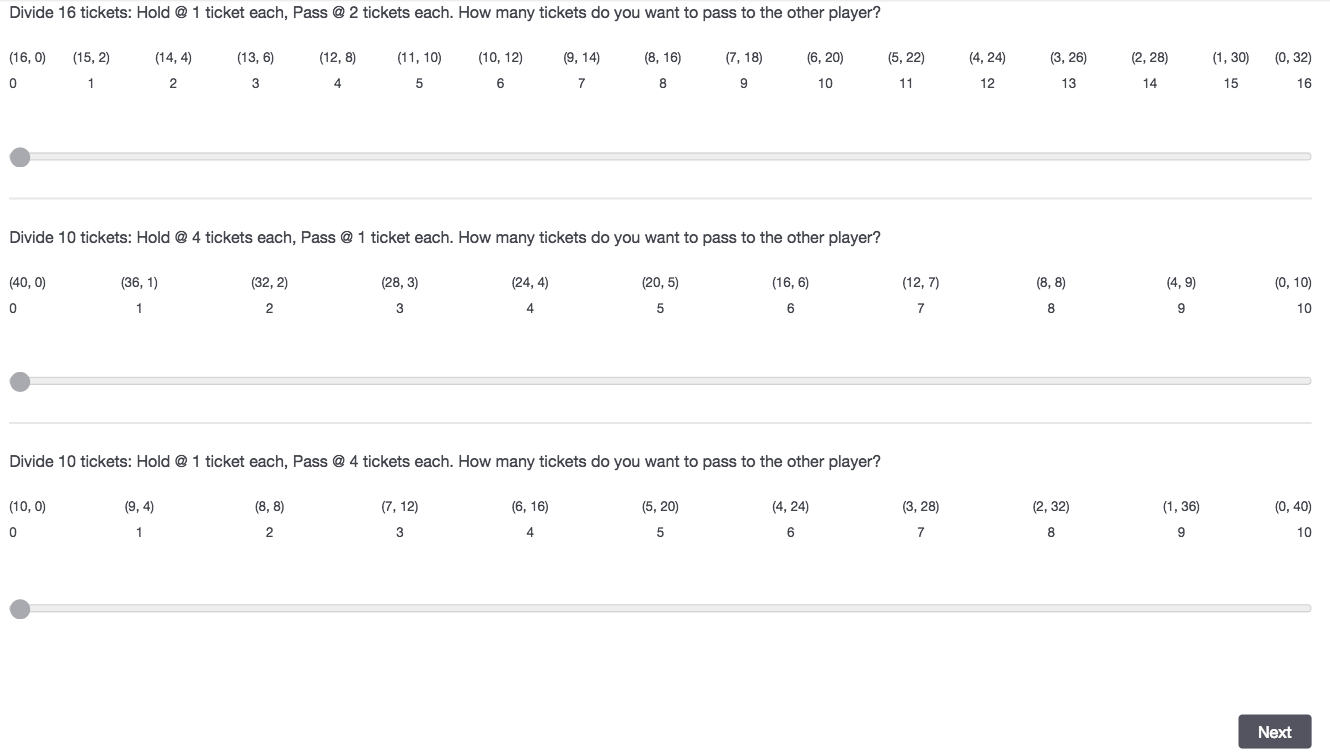
\includegraphics[scale=0.35]{gendict4}\\
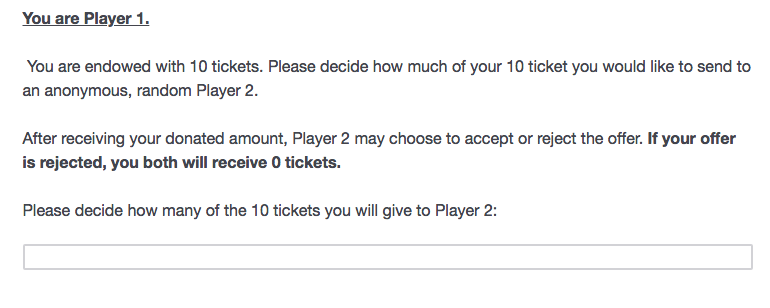
\includegraphics[scale=0.35]{ultimatum1} \\
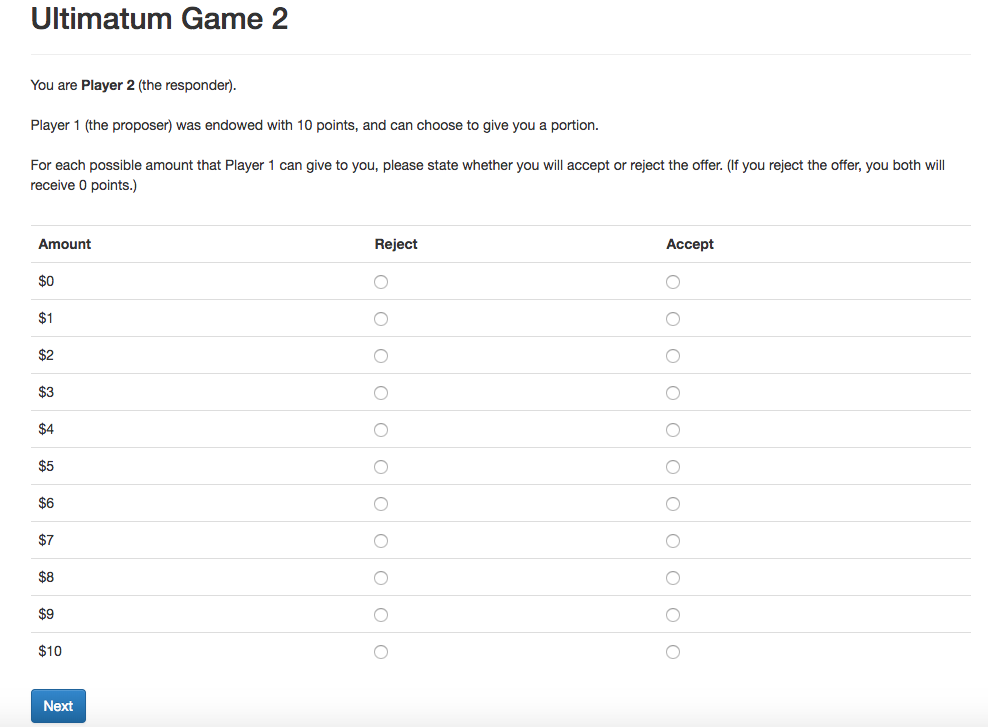
\includegraphics[scale=0.35]{ultimatum2} \\
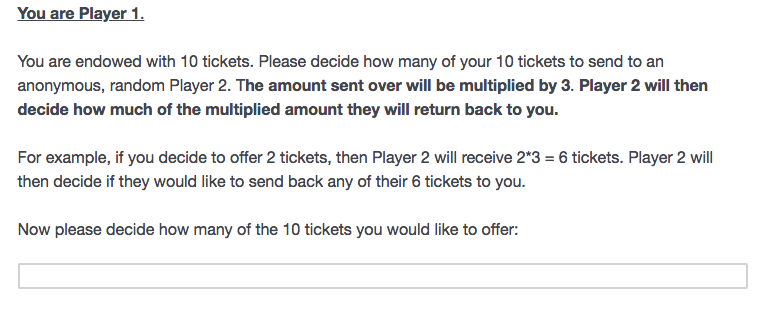
\includegraphics[scale=0.35]{trust1} \\
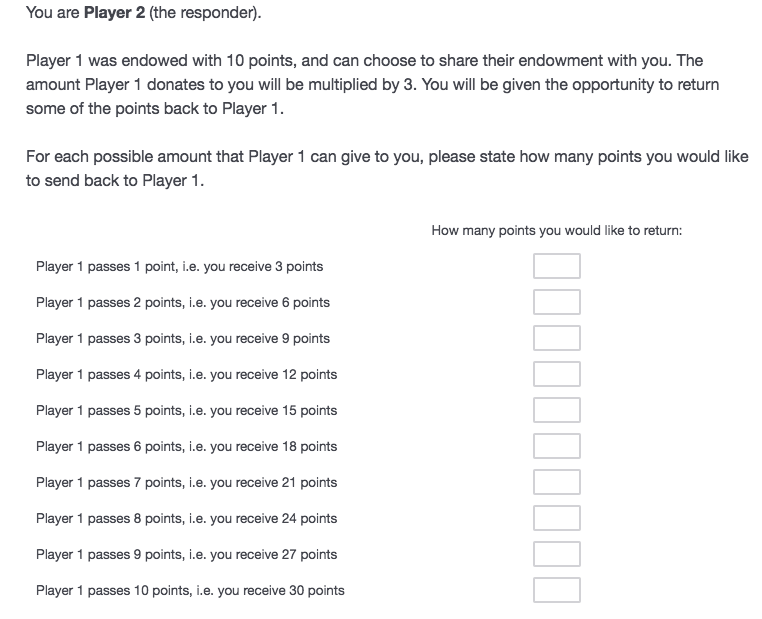
\includegraphics[scale=0.35]{trust2} \\
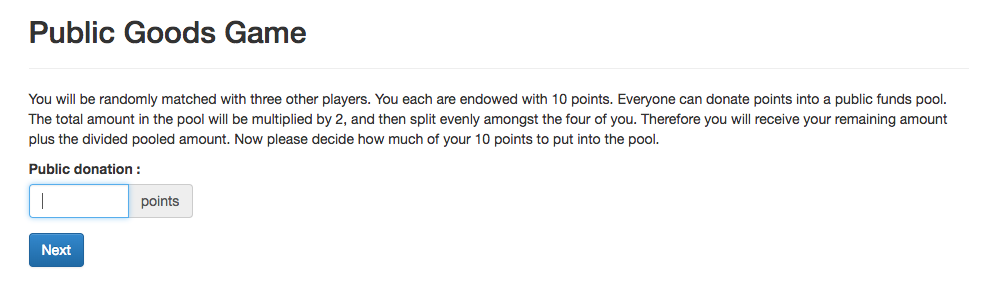
\includegraphics[scale=0.35]{public} \\
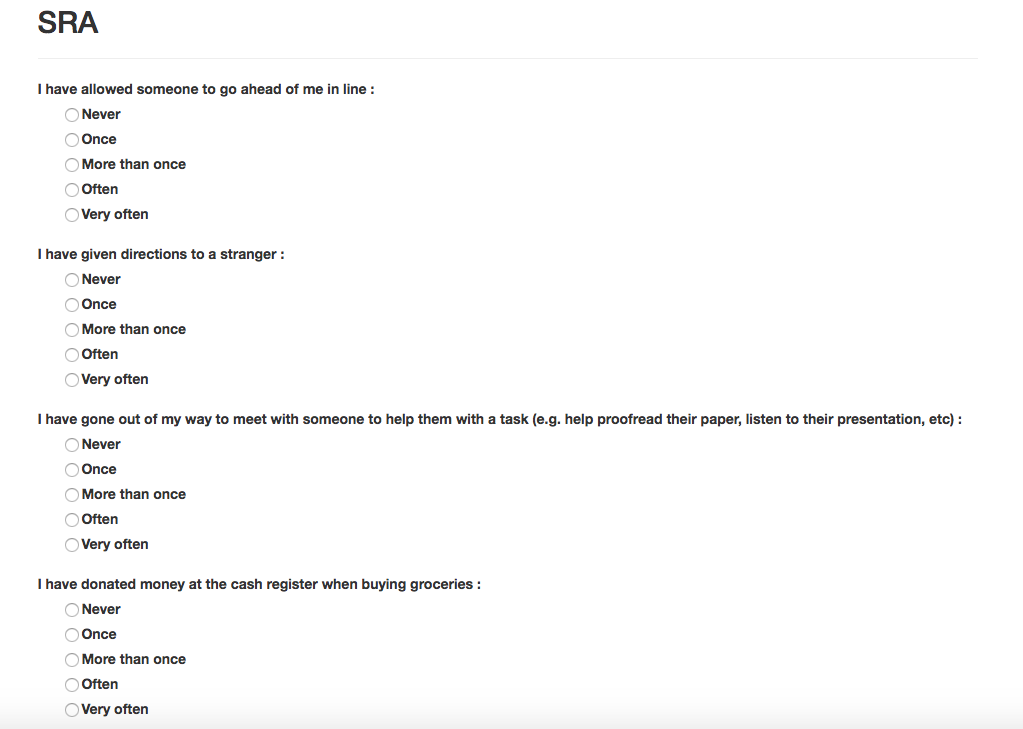
\includegraphics[scale=0.35]{sra} \\




	
\end{document}